\documentclass{article}
\usepackage[utf8]{inputenc}
\usepackage{geometry}
\geometry{hmargin=2.5cm,vmargin=2.5cm}
\usepackage{mathtools} %\usepackage{align}
%\usepackage[french]{babel}
\usepackage{graphicx}

\title{SOD333 - Rapport}
\author{Paul-Antoine Leveilley \& Mila Rocco}
\date{Septembre 2022}

\begin{document}

\maketitle

\begin{center}
Chaque rapport de TP doit faire environ 5 pages.
\end{center}







\newpage
\section{TP1: titre du TP}

\subsection{Introduction}
On étudie la loi d'espérance µ définie ci-dessous, où la fonction de densité q de l'échantillon étudié est inconnue:
$$\mu = \int_0^1 g(x)q(x)dx = \int_0^1 cos(\frac{\pi x}{2})dx\ (=\frac{2}{\pi})$$

 \subsection{Application "brute" de la Méthode de Monte Carlo}
On décide d'étudier l'échantillon $(X_i)_{1\leq i \leq N}$ , qui suit la loi uniforme sur $[0;1]$ afin de vérifier qu'on estime bien µ avec la méthode de Monte Carlo. Sa fonction de densité est donc $q=U([0;1])$. On choisira $N=50$ pour l'étude empirique du problème.

Pour évaluer µ, on applique la méthode de Monte Carlo, et on obtient l'approximation 
$$\hat{\mu}_N = \frac{1}{N} \sum_{i=1}^N g(X_i)$$

- Calculer la variance théorique\\
\begin{align*} 
  Var(\hat{\mu}_N) &= \frac1{N^2} \sum_{i=1}^N Var(g(X_i))\\ 
  &= \frac1{N^2}\times N Var(cos(\frac{\pi X}2)) \\ 
  &= \frac1{N} \left ( \int_0^1 cos^2(\frac{\pi x}2)dx - \left ( \int_0^1 cos(\frac{\pi x}2)dx \right )^2 \right )\\
  &= \frac1{N} \left ( \int_0^1 \frac{1+cos(\pi x)}{2}dx - 
   \frac4{\pi^2} \right )\\
  &= \frac1{N} \left ( \frac{1}{2} - 
   \frac4{\pi^2} \right )\\
  &\approx \frac{0,095}{N}
\end{align*}

- Estimer empiriquement la variance (prendre N = 50)\\
\textbf{résultats du TP.}
On applique la méthode de Monte Carlo et on en tire un échantillon de $NbMC=1000$ tirages.

\begin{figure}[ht]
\centering
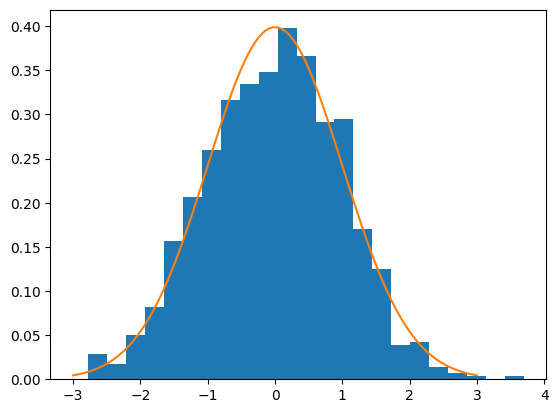
\includegraphics[width=0.4\textwidth]{TP1/MC_brute_TCL.png}
\caption{résultat du TCL}
\end{figure}

\subsection{Echantillonage pondéré}
On génère un nouvel échantillon $(X_i)_{1\leq i \leq N}$ suivant maintenant une fonction d'importance (FI) $\Tilde{q}$ au plus proche de $g(x)$: $X_i \hookrightarrow \Tilde{q}$. Le changement de probabilité donne: 
$$ \hat{\mu}_N = \frac1{N} \sum_{i=1}^N g(X_i)\frac{q(X_i)}{\Tilde{q}(X_i)}\ \overset{p.s.}{\longrightarrow}\ \mu $$

- Chercher une bonne FI\\
(idée: DL au voisinage de 0)  \\
On approxime la fonction g par son développement à l'ordre 2 en 0 (l'ordre 2 ne suffit pas pour que gq et $\Tilde{q}$ gardent le même signe sur $[0,1]$. Rappelons le développement limité en 0 de la fonction cosinus: 
$ cos(x) = 1 - \frac{x^2}{2} + o(x^2) $.
On prend donc pour Fonction d'Importance: 
$$\Tilde{q}_1(x):= 1 - \frac{\pi^2}{8} x^2 $$
Il est important de prendre en compte le fait que $\Tilde{q}$ ne doit pas s'annuler si gq ne s'annule pas. Le DL doit donc être corrigé d'un facteur pour que $\Tilde{q}$ ne devienne pas négatif en $x=1$. En $x=1$, la fonction précédente vaut $\delta = 1 - \frac{\pi^2}{8} < 0$, donc on soustrait $\delta$ à $\Tilde{q}$ pour obtenir notre nouvelle fonction d'importance :
$$\Tilde{q}_2(x):= \frac{\pi^2}{8}(1 - x^2) $$

- Calculer la variance théorique\\
\begin{align*} 
  Var(\hat{\mu}_N) &= \frac1{N^2} \sum_{i=1}^N Var \left ( g(X_i)\frac{q(X_i)}{\Tilde{q}(X_i)}\right)\\ 
  &= \frac1{N} Var\left (\frac{cos(\frac{\pi X}2)}{\frac{\pi^2}{8} (1 - X^2)} \right ) \\ 
  &= \frac1{N} \left ( \int_0^1 \left (\frac{cos(\frac{\pi x}2)}{\frac{\pi^2}{8} (1 -  x^2)} \right )^2dx - \left ( \int_0^1 \frac{cos(\frac{\pi x}2)}{\frac{\pi^2}{8} (1 -  x^2)}dx \right )^2 \right )\\
\end{align*}

\textbf{Application numérique (TP):}

\begin{figure}[ht]
\centering
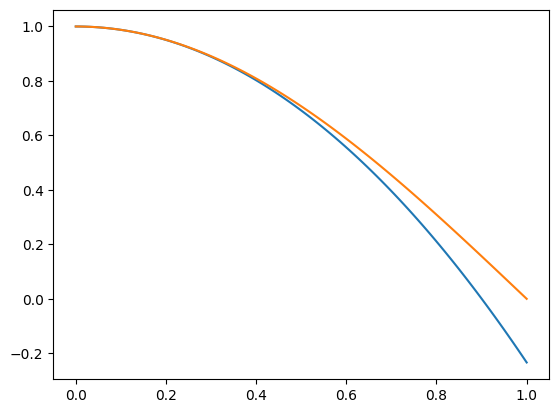
\includegraphics[width=0.4\textwidth]{TP1/DL_ordre2_g.png}
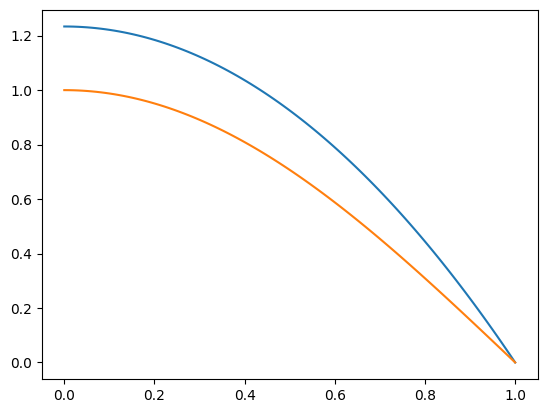
\includegraphics[width=0.4\textwidth]{TP1/DL_ordre2_corrige.png}
\caption{représentation des fonctions gq (en orange) et $\Tilde{q}$ (en bleu): à gauche $\Tilde{q}_1$, à droite $\Tilde{q}_2$}
\end{figure}

\begin{figure}[ht]
\centering
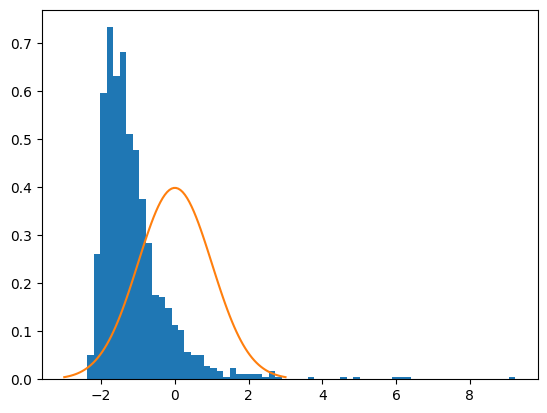
\includegraphics[width=0.4\textwidth]{TP1/IS_TCL_DL_ordre2.png}
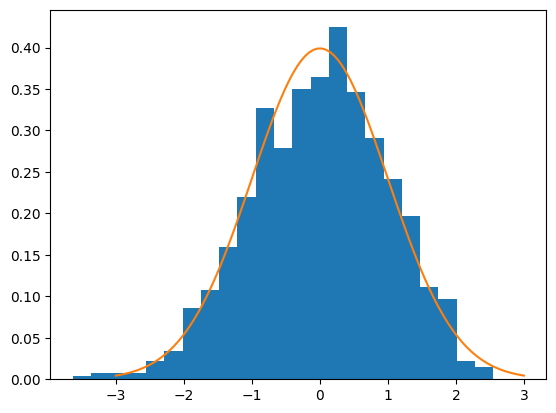
\includegraphics[width=0.4\textwidth]{TP1/IS_TCL_DL_ordre2_corrige.png}
\caption{TCL appliqués respectivement à $\Tilde{q}_1$ (à gauche) et $\Tilde{q}_2$ (à droite)}
\end{figure}

Les résultats du TCL appliqués aux échantillons produits mettent ici en valeur l'importance d'avoir une fonction d'importance du même signe que gq, et que notre développement limité en 0 de gq semble être une bonne approximation pour notre problème.\\

- Utiliser la méthode de rejet pour  générer suivant la FI \\ (Comparer la probabilité d’acceptation théorique à celle obtenue par simulations)\\
On génère un échantillon suivant $p$, et on choisit pour majorant de $g$, $C=1$ tels que 
$$p(x) = \frac{g(x)q(x)}{\int_0^1 g(x)q(x)dx}\ \ \ \ \&\ \ \ \ g(x) \leq C,\ \forall x \in [0;1] $$

Probabilité d'acceptation théorique: 
$$P_a = \frac1C \int_0^1 g(x)q(x)dx 
= \int_0^1 cos(\frac{\pi x}{2})dx 
=\frac{2}{\pi} 
\approx 0,637$$

- Estimer empiriquement la variance.\\
\textbf{application numérique (TP):} On obtient ...

\subsection{Conclusion}
On cherche maintenant à comparer les deux méthodes précédemment appliquées.

- Comparer le rapport des variances des 2 méthodes. Théoriquement et par simulations\\


- Valider par simulations les TCL pour les 2 méthodes en comparant la loi théorique (loi normale) à la loi empirique (histogramme)\\


- Comparer les budgets pour chaque méthode\\


- Calculer la variance de l’estimateur en prenant la FI optimale\\


- Même travail avec $\Tilde{q}=2(1-x)$, ici on simule la FI par la méthode d’inversion de la CDF\\









\newpage
\section{TP2: titre du TP}
\subsection{Introduction}
Dans ce TP, nous allons simuler la trajectoire d'un mobile, et tenter de retrouver ces valeurs grâce à des observations que nous aurons de sa trajectoire.

\begin{figure}[ht]
\centering
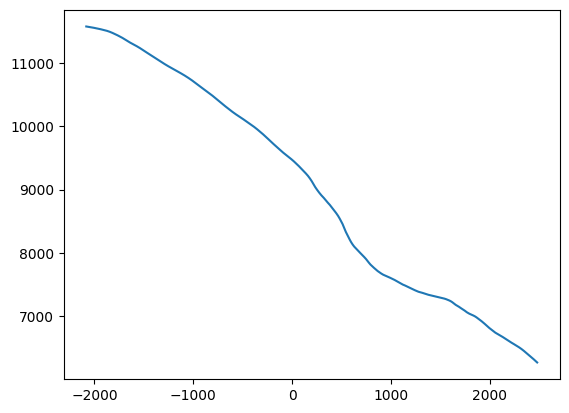
\includegraphics[width=0.4\textwidth]{TP2/position_réelle.png}
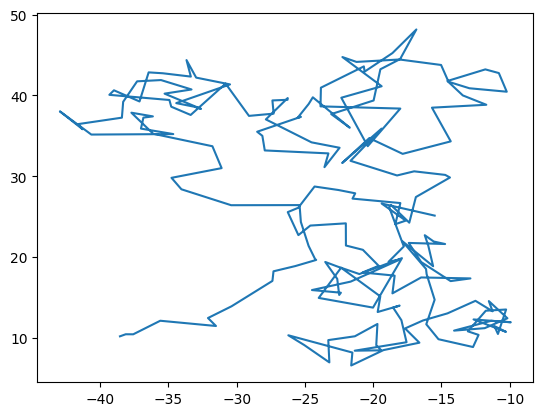
\includegraphics[width=0.4\textwidth]{TP2/vitesse_reelle.png}
\caption{Trajectoire et vitesse associée, que l'on cherche à retrouver}
\end{figure}

\subsection{Titre intermédiaire}
\subsection{Conclusion}

\newpage
\section{TP3: titre du TP}
\subsection{Introduction}
\subsection{Titre intermédiaire}
\subsection{Conclusion}

\newpage
\section{TP4: titre du TP}
\subsection{Introduction}
\subsection{Titre intermédiaire}
\subsection{Conclusion}

\end{document}
